\chapter{Variables Aléatoires Réelles Continues}

\justify

\setlength{\parindent}{0pt}
\renewcommand{\labelitemi}{\textbullet} % Utiliser des points noirs (•)

% ==================================================================================================================================
% Introduction 

On s'intéresse maintenant à des variables aléatoires qui prennent des valeurs réelles mais pas forcément en nombre fini ou dénombrable.
Il est donc nécessaire de définir une probabilité sur $\R$ telle que la probabilité des singletons soit nulle.
Pour cela, nous allons très fortement nous appuyer sur l'intégrale de Lebesgue et la théorie de la mesure. 

% ==================================================================================================================================
% Généralités

\section{Généralités}

\subsection{Vers les variables aléatoires continues}

Dans les chapitres précédents, nous avons vu comment construire, à partir d'univers, des espaces probabilisés 
muni d'une tribu (structure mesurable) et d'une mesure de probabilité. Dans ce cadre probabiliste, une mesure particulière 
joue un rôle significatif sur $\R$ : la \textbf{mesure de Lebesgue}. 

Il est temps maintetant de définir les variables aléatoires réelles continues, c'est à dire, 
des fonctions mesurables dont la loi de probabilité est absolument continue par rapport à la mesure de Lebesgue. 
Intuitivement, cela signifie que nous seront capable de calculer des probabilités par une densité : une fonction intégrable 
positive sur $\R$ dont l'intégrale vaut 1 et permettant de calculer des probabilités par intégration. 

Ceci nécessitera l’introduction de quelques outils d’analyse (densité, intégration, espérance sous forme intégrale), 
qui généraliseront les formules que nous avions pour les lois discrètes.

\subsection{Définitions et propriétés}

\begin{definition}[Variable aléatoire continue]
    Une variable aléatoire $X$ est dite \textbf{continue} si elle peut prendre une infinité non dénombrable de valeurs, typiquement un intervalle de $\R$. 
    C'est donc une application $X : (\Omega, \mathcal{F}) \longrightarrow (\R, \mathcal{B}_\R)$ mesurable. 
        \[ \text{i.e} \quad \forall B \in \mathcal{B}_\R, \quad X^{-1}(B) \in \mathcal{F} \] 
\end{definition}

On peut donc appliquer la mesure de probabilité $\myP$ aux évènements de la forme $\{\omega \in \Omega\}$. 

\begin{definition}[Loi d'une variable aléatoire réelle continue]
    La loi d'une variable aléatoire continue $X$ est définie comme la \textbf{mesure image} de $ \myP$ par $X$ notée 
    $ \myP_X$ telle que : 
        \[ \forall B \in \mathcal{B}_\R, \quad \myP_X(B) = \myP(X^{-1}(B)) = \myP \left( \{\omega \in \Omega \; | \; X(\omega) \in B\} \right) \] 
    Cette loi permet donc de calculer la probabilité que la variable $X$ soit dans un intervalle $[a,b] \subseteq \R$ 
    de la façon suivante : 
        \[ \myP(a < X \leqslant b) = \myP(\{X \in ]a,b]\}) = \myP_X(]a,b]) \]  
\end{definition}

\begin{definition}[Densité de Probabilité]
    Si la mesure $\myP_X$ est absoluement continue par rapport à la mesure de Lebesgue sur $\R$ on dit 
    que $X$ admet une \textbf{densité de probabilité} $ f : \R \longrightarrow \R_+ $ telle que : 
        \[ \forall B \in \mathcal{B}_\R, \quad \myP_X(B) = \int_B f(x) \; dx \] 
\end{definition}


\subsection{Fonction de répartition}

\begin{definition}[Fonction de répartition]
    Soit $X$ une variable aléatoire réelle continue. Sa {fonction de répartition} $F_X$ est définie par :
    \[ F_X : 
        \begin{cases}
            \R \longrightarrow [0,1] \\ 
            a \longmapsto F_X(B) = \myP(X \leqslant a)
        \end{cases} \]
    $F_X$ est une fonction croissante admettant la limite $0$ en $- \infty$ et la 
    limite $1$ en $+ \infty$ et elle est continue à droite. 
\end{definition}

\begin{proposition}[Lien avec la densité]
    Si $X$ admet une densité de probabilité $f$, alors $F_X$ est dérivable et :
        \[
            F_X'(x) = f(x), \quad \text{pour presque tout } x \in \R.
        \]
    On a aussi, pour tout $a < b$ :
        \[
            \myP(a < X \leqslant b) = F_X(b) - F_X(a).
        \]
\end{proposition}

\subsection{Propriétés des variables aléatoires continues}

\begin{definition}[Espérance]
    Soit $X$ une variable aléatoire continue réelle continue de densité $f_X$.
    On appelle espérance de $X$ le nombre 
        \[ \E(X) = \int_{\R} t f_X(t) dt \]
    Si cette intégrale est finie, on dit que l'espérance de $X$ existe. Dans le cas contraire, 
    on dit que la variable aléatoire $X$ n'a pas d'espérance. 
    Autrement dit, on dit que $X$ admet une espérance si l'intégrale $\displaystyle \int_{\R} t f_X(t) \; dt$ 
    est absolument convergente. 
\end{definition}

\begin{theorem}[Formule de Transfert]
    Soit $X$ une variable aléatoire réelle continue de densité $f_X$, et $\varphi : \R \to \R$ une fonction mesurable telle que l’intégrale $\displaystyle \int_{\R} |\varphi(t)| f_X(t) dt$ soit finie. Alors :
        \[ \E(\varphi(X)) = \int_{\R} \varphi (t)f_X(t) dt\]
    Cette formule est une généralisation de l'espérance, on peut par exemple calculer $\E(\ln X)$, $\E(X^2)$, ...
\end{theorem}

\begin{definition}[Variance]
    Soit $X$ une variable aléatoire admettant une espérance. La variance de $X$ est le nombre :
        \[ V(X) = E((X - E(X))^2) = \int_{\R} (t - E(X))^2 f_X(t) \; dt \]
    Toujours comme chez les variables aléatoires réelles discrètes, l'écart-type de $X$ est la racine carrée de $V(X)$ si $V(X)$ existe.
\end{definition}

\begin{theorem}[Koenig-Huyghens]
    Ce théorème permet de calculer plus simplement la variance, à condition que l’espérance $E(X)$ et $E(X^2)$ existent :
        \[ V(X) = E(X^2) - E(X)^2 \]
    C’est souvent la méthode la plus directe pour déterminer la variance d’une variable aléatoire continue.
\end{theorem}


% ==================================================================================================================================
% Principales Lois

\section{Principales Lois}

Définissons maintenant quelques lois fondamentales à connaître par coeur...

\subsection{Loi Uniforme}

\begin{definition}[Loi Uniforme]
    Une variable aléatoire continue $X$ suit une loi uniforme sur $[a,b] \subseteq \R$ lorsque sa densité $f$ 
    est une fonction porte sur l'intervalle $[a,b]$. 
        \[ \text{i.e} \quad f : 
            \begin{cases}
                \R \longrightarrow [0,1] \\ 
                t \longmapsto   \begin{cases}
                                    \frac{1}{b-a} \; \text{si} \; t \in [a,b] \\ 
                                    0 \text{ sinon}
                                \end{cases}
            \end{cases} \] 
    On note alors $X \sim \mathcal{U}([a,b])$. 
\end{definition}

Ces variables aléatoires généralisent la notion d'équiprobabilité dans des espaces continus. 

\begin{proposition}
    Si $X \sim \mathcal{U}([a,b])$, alors la fonction de répartition de $X$ est donnée par : 
        \[ F_X(t) = 
            \begin{cases}
                0 \; \text{si} \; t < a \\ 
                \frac{t-a}{b-a} \; \text{si} \; t \in [a,b] \\ 
                1 \; \text{si} \; t > b 
            \end{cases} \] 
    De plus, on a : 
        \[ \E(X) = \frac{a + b}{2} \quad V(X) = \frac{(b-a)^2}{12} \] 
\end{proposition}


\subsection{Loi Exponentielle}

\begin{definition}[Loi Exponentielle]
    Soit $X$ une variable aléatoire continue. On dit que $X$ suit une loi exponentielle de paramètre $ \lambda > 0$ 
    si sa densité de probabilité est de la forme : 
        \[ f : 
            \begin{cases}
                \R \longrightarrow [0,1] \\ 
                t \longmapsto 
                    \begin{cases}
                        \lambda e^{-\lambda t} \; \text{si} \; t \geqslant 0 \\ 
                        0 \; \text{si} \; t \leqslant 0 
                    \end{cases}
            \end{cases} \] 
    On note alors $X \sim \mathcal{E}(\lambda)$. 
\end{definition}

Une loi exponentielle modélise la durée de vie d'une phénomène sans mémoire. Autrement dit, elle mesure la probabilité 
d'une phénomène ait duré pendant $t$ unités de temps. 

\begin{proposition}
    Si $X \sim \mathcal{E}(\lambda)$, alors sa fonction de répartition est donnée par : 
        \[ F_X(t) = 
            \begin{cases}
                1 - e ^{- \lambda t } \; \text{si} t \geqslant 0 \\ 
                0 \; \text{si} \; t < 0 
            \end{cases} \] 
    De plus, on a : 
        \[ \E(X) = \frac{1}{\lambda} \quad V(X) = \frac{1}{\lambda^2} \] 
\end{proposition}

\begin{figure}[h]
    \centering
    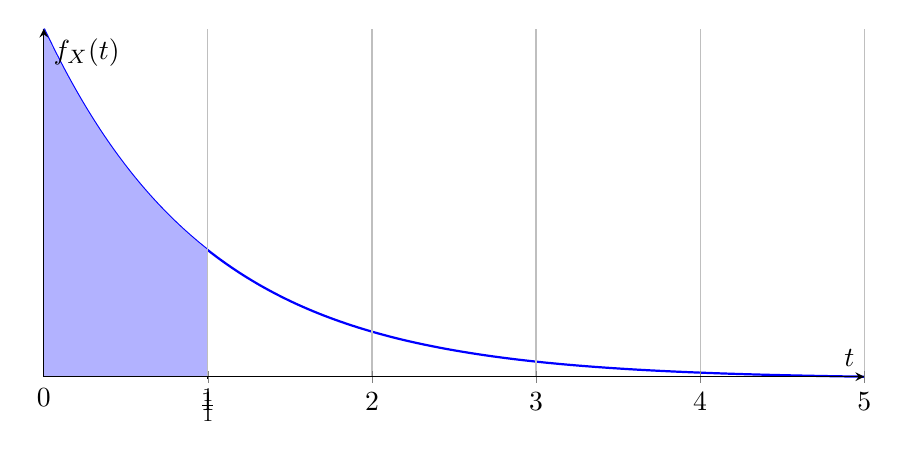
\begin{tikzpicture}
        \begin{axis}[
            domain=0:5,
            samples=100,
            axis lines=middle,
            xlabel=$t$,
            ylabel={$f_X(t)$},
            xtick={0,1,2,3,4,5},
            ytick=\empty,
            height=6cm,
            width=12cm,
            enlargelimits=false,
            clip=false,
            axis on top,
            grid=major,
        ]
            % Paramètre lambda
            \def\lambda{1}

            % Courbe de densité exponentielle
            \addplot [
                thick,
                blue,
                smooth
            ] {\lambda * exp(-\lambda * x)};

            % Zone entre 0 et espérance = 1/lambda
            \addplot [
                domain=0:1,
                samples=50,
                fill=blue!30,
                draw=none
            ] {\lambda * exp(-\lambda * x)} \closedcycle;

            % Lignes verticales
            \draw[dashed] (axis cs:1,0) -- (axis cs:1,{exp(-1)});
            \node[below] at (axis cs:1,0) {$\frac{1}{\lambda}$};
            \node[below] at (axis cs:0,0) {$0$};
        \end{axis}
    \end{tikzpicture}
    \caption{Densité de probabilité de la loi exponentielle $\mathcal{E}(\lambda)$ avec espérance $\frac{1}{\lambda}$}
\end{figure}



\subsection{Loi Normale}

\begin{definition}[Loi Normale]
    Soit $X$ une variable aléatoire continue. On dit que $X$ suit une loi normale de paramètres $\mu \in \R$ et $\sigma > 0$ 
    si sa densité de probabilité est donnée par : 
        \[ f : 
            \begin{cases}
                \R \longrightarrow \R^+ \\
                t \longmapsto \dfrac{1}{\sigma \sqrt{2\pi}} \exp\left( -\dfrac{(t - \mu)^2}{2\sigma^2} \right)
            \end{cases} \]
    On note alors $X \sim \mathcal{N}(\mu, \sigma^2)$. 
\end{definition}

La loi normale est très utilisée pour modéliser des phénomènes aléatoires centrés autour d'une moyenne $\mu$, 
avec une variabilité mesurée par l’écart-type $\sigma$. Elle est également appelée loi de Gauss.

\begin{proposition}
    Si $X \sim \mathcal{N}(\mu, \sigma^2)$, alors :
        \[ \E(X) = \mu \quad \text{et} \quad V(X) = \sigma^2 \]
    Sa fonction de répartition $F_X(t) = \mathbb{P}(X \leqslant t)$ n’a pas d’expression simple à l’aide de fonctions élémentaires. On utilise donc souvent la loi normale centrée réduite :
        \[ Z \sim \mathcal{N}(0, 1) \]
    avec densité : 
        \[ f_Z(t) = \dfrac{1}{\sqrt{2\pi}} e^{-t^2/2} \]
    et on a :
        \[ \mathbb{P}(X \leqslant t) = \mathbb{P}\left(Z \leq \dfrac{t - \mu}{\sigma}\right) \]
\end{proposition}

\begin{figure}[h]
    \centering
    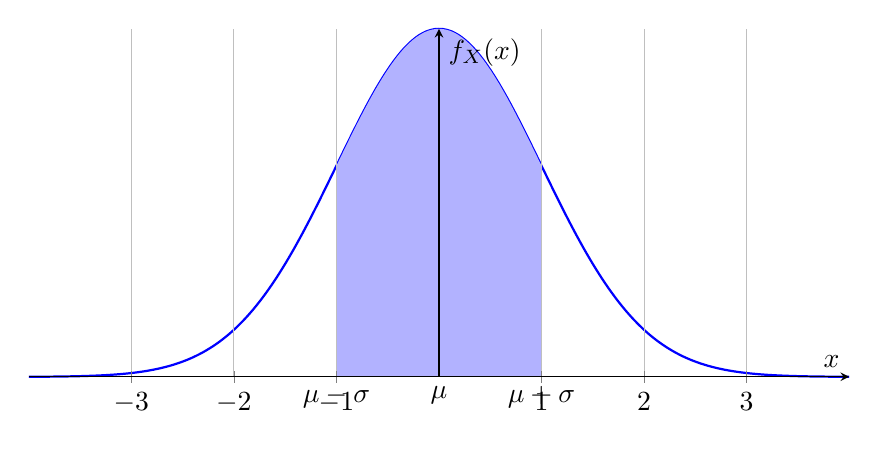
\begin{tikzpicture}
        \begin{axis}[
            domain=-4:4,
            samples=100,
            axis lines=middle,
            xlabel=$x$,
            ylabel={$f_X(x)$},
            xtick={-3,-2,-1,0,1,2,3},
            ytick=\empty,
            height=6cm,
            width=12cm,
            enlargelimits=false,
            clip=false,
            axis on top,
            grid = major,
        ]
            % Densité normale centrée réduite
            \addplot [thick, blue, smooth] {1/sqrt(2*pi) * exp(-x^2/2)};
            
            % Zone entre -1 et 1 (mu - sigma, mu + sigma)
            \addplot [
                domain=-1:1, 
                samples=50,
                fill=blue!30,
                draw=none
            ] {1/sqrt(2*pi) * exp(-x^2/2)} \closedcycle;
            
            % Lignes verticales pour mu-sigma et mu+sigma
            \draw[dashed] (axis cs:-1,0) -- (axis cs:-1,0.25);
            \draw[dashed] (axis cs:1,0) -- (axis cs:1,0.25);
            
            % Flèche vers mu
            \node[below] at (axis cs:0,0) {$\mu$};
            \node[below] at (axis cs:-1,0) {$\mu - \sigma$};
            \node[below] at (axis cs:1,0) {$\mu + \sigma$};
        \end{axis}
    \end{tikzpicture}
    \caption{Densité de probabilité d'une loi normale $\mathcal{N}(\mu, \sigma^2)$ avec mise en évidence de l'intervalle $[\mu - \sigma, \mu + \sigma]$}
\end{figure}

\subsection{Loi de Cauchy}

\begin{definition}[Loi de Cauchy]
    Une variable aléatoire $X$ suit une loi de Cauchy de paramètre $x_0 \in \R$ (localisation) et $\gamma > 0$ (échelle) si :
        \[ f(t) = \frac{1}{\pi \gamma} \cdot \frac{1}{1 + \left( \frac{t - x_0}{\gamma} \right)^2} \]
    On note $X \sim \mathcal{C}(x_0, \gamma)$.
\end{definition}

La loi de Cauchy est une loi sans espérance ni variance, utilisée en physique (résonances).

\begin{proposition}
    La fonction de répartition de $X \sim \mathcal{C}(x_0, \gamma)$ est :
        \[ F_X(t) = \frac{1}{\pi} \arctan\left( \frac{t - x_0}{\gamma} \right) + \frac{1}{2} \]
\end{proposition}


\subsection{Loi Gamma}

\begin{definition}[Loi Gamma]
    Une variable aléatoire $X$ suit une loi Gamma de paramètres $k > 0$ (forme) et $\lambda > 0$ (taux) si :
        \[ f(t) = 
            \begin{cases}
                \dfrac{\lambda^k}{\Gamma(k)} t^{k-1} e^{-\lambda t} & \text{si } t \geq 0 \\
                0 & \text{sinon}
            \end{cases} \]
    On note $X \sim \Gamma(k, \lambda)$.
\end{definition}

La loi Gamma modélise des durées de vie cumulées (somme de $k$ exponentielles).

\begin{proposition}
    \[ \E(X) = \frac{k}{\lambda} \quad V(X) = \frac{k}{\lambda^2} \]
\end{proposition}


\subsection{Loi de Rayleigh}

\begin{definition}[Loi de Rayleigh]
    Une variable aléatoire $X$ suit une loi de Rayleigh de paramètre $\sigma > 0$ si sa densité est :
        \[ f(t) = 
            \begin{cases}
                \dfrac{t}{\sigma^2} e^{-t^2 / (2 \sigma^2)} & \text{si } t \geq 0 \\
                0 & \text{sinon}
            \end{cases} \]
    On note $X \sim \mathcal{R}(\sigma)$.
\end{definition}

\begin{proposition}
    \[ \E(X) = \sigma \sqrt{\dfrac{\pi}{2}} \quad V(X) = \left(2 - \dfrac{\pi}{2} \right)\sigma^2 \]
\end{proposition}

\subsection{Loi $\chi^2$}

\begin{definition}[Loi $\chi^2$]
    Une variable aléatoire $X$ suit une loi $\chi^2$ à $\nu \in \N^*$ degrés de liberté si :
        \[ X \sim \Gamma\left(\frac{\nu}{2}, \frac{1}{2}\right) \]
    Soit :
        \[ f(t) = 
            \begin{cases}
                \dfrac{1}{2^{\nu/2} \Gamma(\nu/2)} t^{\nu/2 - 1} e^{-t/2} & \text{si } t \geq 0 \\
                0 & \text{sinon}
            \end{cases} \]
\end{definition}

\begin{proposition}
    \[ \E(X) = \nu \quad V(X) = 2\nu \]
\end{proposition}


\begin{table}[h]
    \centering
    \renewcommand{\arraystretch}{1.4}
    \begin{tabularx}{\textwidth}{|c|c|X|c|c|}
        \hline
        \textbf{Loi} & \textbf{Notation} & \textbf{Densité $f(t)$} & \textbf{$\E(X)$} & \textbf{$V(X)$} \\
        \hline

        Uniforme & $\mathcal{U}([a,b])$ & 
        $f(t) = \begin{cases}
            \frac{1}{b-a} & t \in [a,b] \\
            0 & \text{sinon}
        \end{cases}$ & 
        $\dfrac{a + b}{2}$ & 
        $\dfrac{(b-a)^2}{12}$ \\
        \hline

        Exponentielle & $\mathcal{E}(\lambda)$ & 
        $f(t) = \begin{cases}
            \lambda e^{-\lambda t} & t \geq 0 \\
            0 & \text{sinon}
        \end{cases}$ & 
        $\dfrac{1}{\lambda}$ & 
        $\dfrac{1}{\lambda^2}$ \\
        \hline

        Normale & $\mathcal{N}(\mu, \sigma^2)$ & 
        $f(t) = \dfrac{1}{\sigma \sqrt{2\pi}} e^{ - \frac{(t - \mu)^2}{2\sigma^2} }$ & 
        $\mu$ & 
        $\sigma^2$ \\
        \hline

        Cauchy & $\mathcal{C}(x_0, \gamma)$ & 
        $f(t) = \dfrac{1}{\pi \gamma} \cdot \dfrac{1}{1 + \left( \frac{t - x_0}{\gamma} \right)^2}$ & 
        -- & 
        -- \\
        \hline

        Gamma & $\Gamma(k, \lambda)$ & 
        $f(t) = \begin{cases}
            \dfrac{\lambda^k}{\Gamma(k)} t^{k-1} e^{-\lambda t} & t \geq 0 \\
            0 & \text{sinon}
        \end{cases}$ & 
        $\dfrac{k}{\lambda}$ & 
        $\dfrac{k}{\lambda^2}$ \\
        \hline

        Rayleigh & $\mathcal{R}(\sigma)$ & 
        $f(t) = \begin{cases}
            \dfrac{t}{\sigma^2} e^{ -\frac{t^2}{2\sigma^2} } & t \geq 0 \\
            0 & \text{sinon}
        \end{cases}$ & 
        $\sigma \sqrt{\dfrac{\pi}{2}}$ & 
        $\left( 2 - \dfrac{\pi}{2} \right) \sigma^2$ \\
        \hline

        Khi-deux & $\chi^2(\nu)$ & 
        $f(t) = \begin{cases}
            \dfrac{1}{2^{\nu/2} \Gamma(\nu/2)} t^{\nu/2 - 1} e^{-t/2} & t \geq 0 \\
            0 & \text{sinon}
        \end{cases}$ & 
        $\nu$ & 
        $2\nu$ \\
        \hline

    \end{tabularx}
    \caption{Résumé des lois de probabilité continues usuelles}
\end{table}

